\chapter{Inleiding}
\label{inleiding}
%%%%%%%%%%%%%%%%%%%%%%%%%%%%%%%%%%%%%%%%%%%%%%%%%%%%%
%          Waarom configuratiemanagement?           %
%%%%%%%%%%%%%%%%%%%%%%%%%%%%%%%%%%%%%%%%%%%%%%%%%%%%%
Configuratiebeheergereedschappen zijn ontwikkeld om het leven van systeembeheerders makkelijker te maken.
De serverinfrastructuren die ze moeten onderhouden worden steeds uitgebreider en complexer.
Manueel elke server configureren kost niet alleen te veel tijd, maar is ook erg foutgevoelig.\cite{why_do_upgrades_fail}
Er bestaan reeds verschillende oplossingen voor dit probleem:
een eerste manier is het gebruik van scripts.
Dit automatiseert al een deel van het werk, maar heeft ook een belangrijk nadeel:
als de uitvoering van een script afgebroken wordt blijft het systeem in een onstabiele toestand.\cite{sysadvent}

Een tweede manier om een verzameling gelijkaardige machines van hun initi\"ele configuratie te voorzien is het gebruik van images.
Daarbij wordt eerst \'e\'en machine manueel geconfigureerd en daarna wordt de volledige set-up gekloond naar de rest van de servers.
Deze methode werkt niet meer voor het verdere onderhoud van de machines.

%%%%%%%%%%%%%%%%%%%%%%%%%%%%%%%%%%%%%%%%%%%%%%%%%
%          Overgaan naar de cloud               %
%%%%%%%%%%%%%%%%%%%%%%%%%%%%%%%%%%%%%%%%%%%%%%%%%
Dit onderhoudsprobleem komt nog prominenter voor als de infrastructuur niet lokaal maar in de cloud gehost wordt.
Een groot voordeel van werken in de cloud is de flexibiliteit waarmee servers kunnen toegevoegd en weggenomen worden.
Dit proces gebeurt vaak automatisch waardoor manuele configuratie helemaal geen optie meer is.
In een dergelijke omgeving is een tool die uit zichzelf de volledige infrastructuur kan beheren bijna een noodzaak. \cite{opening_the_clouds,deploying_elastic_services}

%%%%%%%%%%%%%%%%%%%%%%%%%%%%%%%%%%%%%%%%%%%%%
%          Werking huidige tools            %
%%%%%%%%%%%%%%%%%%%%%%%%%%%%%%%%%%%%%%%%%%%%%
Configuratiebeheergereedschappen (of CMS: Configuration Management Software, vanaf nu zal deze term gebruikt worden) zoals Ansible\cite{ansible}, Puppet\cite{puppet}, CFEngine\cite{cfengine},\ldots laten toe op een effici\"ente manier IT-infrastructuren op te zetten en te onderhouden.
De gebruiker van een dergelijke tool specifi\"eert eerst een model dat de gewenste toestand van de volledige infrastructuur beschrijft.
Dit model bestaat uit een oplijsting van machines met de gewenste aanwezige resources (bestanden, mappen, services,\ldots) die ze moeten aanbieden.
Sommige tools laten ook toe samenhorende resources te groeperen in een concept, zoals een webserver of een databaseserver.
Dit vermijdt duplicatie van code in het model.

Bij het uitrollen van een model (een "deployment run") inspecteert de CMS de huidige toestand van elke machine en vergelijkt ze met de gewenste toestand.
Als er een verschil is maakt de CMS de nodige aanpassingen, indien niet onderneemt ze geen actie.
De beheerder van de verzameling systemen moet na het opstellen van de initi\"ele configuratie zelf geen stappen meer ondernemen om te verzekeren dat de gewenste situatie bereikt wordt.
Als er later nog aanpassingen moeten gebeuren moet enkel het model aangepast worden en een nieuwe deployment run gestart worden.

%%%%%%%%%%%%%%%%%%%%%%%%%%%%%%%%%%%%%%%%%%%%%%%%%%%%%
%          Dependencies gebruiken gaat beter        %
%%%%%%%%%%%%%%%%%%%%%%%%%%%%%%%%%%%%%%%%%%%%%%%%%%%%%
Een belangrijk aspect van elk gedistribueerd systeem zijn de afhankelijkheden die bestaan tussen de verschillende onderdelen.
Stel het voorbeeld van een LAMP-stack: een Linuxdistributie met de Apache webserver, de MySQL database en PHP.
Daar kan de webserver niet zijn volledige functionaliteit aanbieden voordat de database online is.
De webserver is dus afhankelijk van de databaseserver.
Zolang PHP niet ge\"installeerd is kan de webserver ook geen dynamische pagina's aanbieden.
Ze is dus ook afhankelijk van de PHP-installatie. \todo{Is PHP een vereiste of een afhankelijkheid? Vereiste definieren als altijd binnen 1 host?}
Een volledige mapping van de verschillende afhankelijkheden binnen de LAMP-stack is te zien op figuur \ref{fig:lamp_dep}.

\begin{figure}[h]
    \begin{center}
    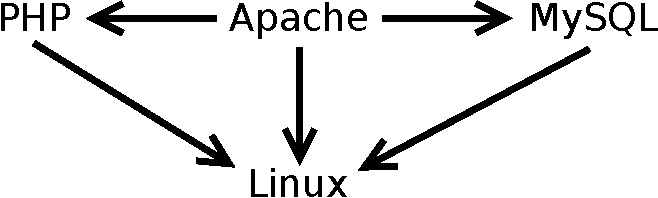
\includegraphics[width=0.6\textwidth]{images/lamp_dep.pdf}
    \caption{Grafische voorstelling van de afhankelijkheden binnen een LAMP-stack}
    \label{fig:lamp_dep}
    \end{center}
\end{figure}

Als deze afhankelijkheden niet gespecificeerd worden in het model kan de CMS er ook geen rekening mee houden.
Het kan dat de tool het model in een foute volgorde uitrolt: eerst de webserver, dan PHP en uiteindelijk de database.
De webserver zal bij het opstarten proberen te verbinden met de database, maar deze is nog niet online.
In de tijd tussen het opstarten van de webserver en de installatie van PHP zal ze ook geen dynamische webpagina's kunnen tonen.
Een op het eerste zicht succesvolle deployment run kan dus leiden tot een configuratie die niet volledig werkt.

In vergelijking met de beginsituatie is de toestand van de configuratie na de ene run wel al minder afwijkend van de gewenste situatie:
de verschillende pakketten, services en configuratiebestanden zijn al aanwezig.
Tijdens de volgende deployment run zal de Apache service herstart worden en dan zal ze wel kunnen connecteren met de database.


%Databases en webservers zijn abstracties die bestaan uit een verzameling basisobjecten zoals bestanden, pakketten en services.\todo{Beter woord voor abstracties}
%Tussen deze objecten bestaan er natuurlijk ook afhankelijkheden, bijvoorbeeld tussen een bestand en de map waarin het staat:
%als de CMS eerst probeert het bestand te cree\"eren en dan pas de map zal de deployment run slechts gedeeltelijk slagen want een bestand kan niet bestaan
%zonder een bovenliggende map.
%Figuur \ref{fig:file_dir_dep} stelt deze afhankelijkheid nog eens grafisch voor.
%
%\begin{figure}
%    \begin{center}
%    
\includegraphics[width=0.6\textwidth]{images/file_dir_dep.pdf}
%    \caption{Grafische voorstelling van de afhankelijkheid tussen een bestand en zijn bovenliggende folder}
%    \label{fig:file_dir_dep}
%    \end{center}
%\end{figure}

In tegenstelling tot het voorbeeld van de LAMP-stack zal de gebruiker direct na het uitrollen al zien dat er iets foutgaat.
De CMS zal namelijk melden dat sommige resources niet werden uitgerold.
Bij de LAMP-stack werd alles succesvol uitgerold, maar de gebruiker kan pas zien dat er iets fout is als hij de logs van de Apache service bekijkt, of probeert een site te bezoeken.

We maken dus het onderscheid tussen twee gevallen: vereisten en afhankelijkheden.
In het geval van het bestand en de map is er sprake van een \textit{vereiste} die niet voldaan is: de map moet bestaan v\'o\'or het aanmaken van het bestand of deze wordt niet aangemaakt.
In het geval van de LAMP-stack houdt de CMS geen rekening met de \textit{afhankelijkheid} tussen de webserver en de databaseserver.
Alle resources worden foutloos aangemaakt en opgestart, maar toch werkt de uiteindelijke configuratie niet omdat een foute volgorde werd gehanteerd.
In beide gevallen is een extra deployment run nodig voordat de configuratie correct werkt.

CMS zal nooit aanpassingen maken die zorgen voor een configuratie die verder afwijkt van het model dan voorheen.
Na een paar iteraties zal uiteindelijk altijd de gewenste configuratie bereikt worden. 
Grafisch wordt dit voorgesteld op figuur \ref{fig:convergentie}.
Het aantal iteraties is afhankelijk van de hoeveelheid afhankelijkheden en vereisten die bestaan, maar niet aanwezig zijn in het model.

\begin{figure}
    \begin{center}
    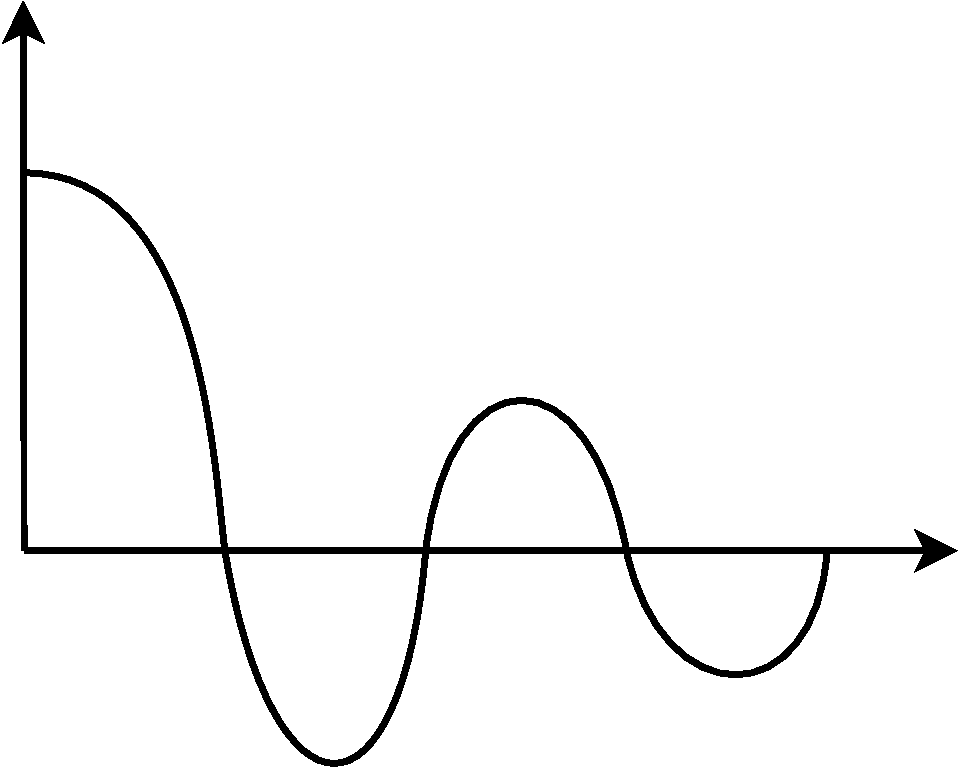
\includegraphics[width=0.6\textwidth]{images/convergentie.pdf}
    \caption{Grafische voorstelling van de convergentie na een reeks deployment runs.}
    \label{fig:convergentie}
    \end{center}
\end{figure}

Als de CMS weet heeft van de afhankelijkheden en vereisten kan het aantal uitrolmomenten drastisch verminderd worden.

%%%%%%%%%%%%%%%%%%%%%%%%%%%%%%%%%%%%%%%%%%%%%%%%%%%%%
%          Afhankelijkheden met huidige tools       %
%%%%%%%%%%%%%%%%%%%%%%%%%%%%%%%%%%%%%%%%%%%%%%%%%%%%%
De huidige CMS laten toe om op het niveau van bestanden, packages en services vereisten en afhankelijkheden te specificeren.
De specificatie van een vereiste en een afhankelijkheid overlapt bij deze tools en wordt een ``requirement'' genoemd.
Bij het uitrollen van een model gebruikt de software die informatie om een volgorde op te leggen waarmee de verschillende objecten aangemaakt worden.

Deze tools compileren tijdens de deployment voor elke machine hun deel van het model.
Elke machine heeft dus enkel weet van de eigen resources, en er is ook geen communicatie tussen machines onderling.
Afhankelijkheden en vereisten binnen eenzelfde machine verwerken is geen probleem, maar tussen verschillende machines is dit niet mogelijk.
Als de LAMP-stack op \'e\'en machine ge\"installeerd wordt kan de gebruiker nog aangeven dat de Apache service afhankelijk is van de databaseservice en PHP.
Als daarintegen de Apache service op een machine draait en de MySQL-service op een andere kan de gebruiker dit met de huidige tools niet meer aangeven.
De enige optie is dan meerdere keren het model uitrollen tot de configuratie correct werkt.
\footnote{Voor Puppet bestaat er wel een workaround, zie \cite{puppet-orchestration}. ``Orchestration'' CMS zoals Ansible\cite{ansible} kan dit wel. \todo{Verschil opzoeken en uitleggen hier of in related works?}}

%%%%%%%%%%%%%%%%%%%%%%%%%%%%%%%%%%%%%%%%%%%%%%%%%%%%%
%     Afhankelijkheden en vereisten met IMP         %
%%%%%%%%%%%%%%%%%%%%%%%%%%%%%%%%%%%%%%%%%%%%%%%%%%%%%
IMP (Infrastructure Management Platform)\cite{IMP} is een nieuwe tool die momenteel nog in ontwikkeling is.
Ze verschilt op twee vlakken van de andere CMS.

Ten eerste kan de gebruiker naast vereisten ook relaties specificeren.
Deze relaties worden gedefini\"eerd tussen twee entiteiten. 
Entiteiten in IMP zijn de klasses uit een objectgerichte programmeertaal, en resources zijn de instanties van dergelijke klasses.
Relaties gelden dus voor alle instanties van een entiteit, in tegenstelling tot vereisten die tussen twee specifiece resources gespecificeerd worden.
De gebruiker kan zelf aangeven of een relatie al dan niet afhankelijk is.

Ten tweede krijgt elke machine tijdens het uitrolproces het volledige model ter beschikking en niet alleen zijn eigen deel.
De verschillende machines wisselen ook berichten met elkaar uit over de resources die ze al uitgerold hebben.
Machines kunnen zo niet alleen rekening houden met afhankelijkheden en vereisten tussen eigen resources, maar ook met andere machines.

Deze twee eigenschappen samen zorgen ervoor dat in IMP afhankelijkheden tussen samengestelde entiteiten die op verschillende machines gedefini\"eerd zijn verwerkt kunnen worden.
Een voorbeeld hiervan is de afhankelijkheid tussen de webserver en databaseserver uit de gedistribueerde versie van de LAMP-stack.
Deze kan niet gemodelleerd worden in de andere CMS. 

%%%%%%%%%%%%%%%%%%%%%%%%%%%%%%%%%%%%%%%%%%%%%%%%%%%%%
%          Probleem/doelstelling                    %
%%%%%%%%%%%%%%%%%%%%%%%%%%%%%%%%%%%%%%%%%%%%%%%%%%%%%
Het is duidelijk dat het belangrijk is om alle relaties (zowel afhankelijkheden en vereisten) die aanwezig zijn tussen resources van een gedistribueerde infrastructuur expliciet te vermelden in het configuratiemodel.
Deze thesis onderzoekt hoe aan de hand van heuristieken automatisch deze relaties kunnen toegevoegd worden aan het configuratiemodel.
Dit vermindert de moeite die gebruiker van de software moet doen bij het opstellen van het model, en vermindert mogelijks het aantal fouten dat gebeurt tijdens het uitrollen.
Daartegenover staat wel dat als de gebruiker alle functionaliteit van IMP wil benutten hij/zij ook de relaties tussen de gedefini\"eerde entiteiten zal moeten specifi\"eren.

Als IMP een optimale volgorde gebruikt bij het uitrollen van een model kan na \'e\'en uitrolproces een volledig functionerende infrastructuur opgestart worden.
Elke uitrolvolgorde die resulteert in een volledig werkende configuratie na \'e\'en uitrolmoment wordt als optimaal aanzien.

De veronderstelling is wel dat degene die het model opstelt genoeg domeinspecifieke informatie aanlevert die door deze heuristieken gebruikt kan worden.
\todo{Belang van correct uitrollen: kan soms interessanter zijn dan snel uitrollen}
